%   % !TEX root = ../../VIII,3_Rahmen-TeX_8-1.tex
%
%
%   Band VIII, 3 N.~??A21.2/Y.5
%   Signatur/Tex-Datei: LH_37_03_118r
%   RK-Nr. 60207
%   Überschrift: De duabus tabulis planis divellendis
%   Datierung: [März/April 1683]
%   WZ: (keins)
%.  SZ: (keins)
%.  Bilddateien (PDF): LH037_03_118r_d (insgesamt: eine)
%
%
\selectlanguage{ngerman}%
\frenchspacing%
%
\begin{ledgroupsized}[r]{120mm}
\footnotesize
\pstart
\noindent\textbf{Überlieferung:}
\pend
\end{ledgroupsized}
\begin{ledgroupsized}[r]{114mm}
\footnotesize
\pstart \parindent -6mm
\makebox[6mm][l]{\textit{L}}%
Konzept: LH~XXXVII~3 Bl.~118.
Ein Blatt~8\textsuperscript{o}.
Eine Seite auf Bl.~118~r\textsuperscript{o};
Bl.~118~v\textsuperscript{o} 
überliefert das Konzept \textit{L\textsuperscript{1}} von \textit{LSB} III, 3 N.~456\cite{01262} (Brief an E.~Mariotte von März/April 1683).
Am unteren Rand von Bl.~118~r\textsuperscript{o} gestrichenes gegenläufiges Satzfragment von Leibnizens Hand:
\textit{cette fois vous n'en aures pas jugé l'usage necessaire}
(möglicherweise mit dem Briefkonzept auf der Rückseite zusammenhängend).
Der Textabschnitt \textit{Experientia notum} \lbrack...\rbrack\ \textit{aere libero} (S.~\refpassage{LH037_03_118r_wiedergabe-1}{LH037_03_118r_wiedergabe-2}) ist von N.~14\textsubscript{2} (S.~\refpassage{LH_37_03_069r_duaetabulae-1}{LH_37_03_069r_duaetabulae-2}) abgeschrieben.
% Kein Wasserzeichen.
\pend
\end{ledgroupsized}
%
%
\selectlanguage{latin}%
\frenchspacing%
%
%
\count\Bfootins=1100
\count\Afootins=1100
\count\Cfootins=1100
\vspace{8mm}
\pstart%
\normalsize%
\noindent%
%
\lbrack118~r\textsuperscript{o}\rbrack\ % Blatt 118r
%
\pend%
% Überschrift
\pstart%
\centering%
De duabus tabulis planis in loco clauso aqua pleno divellendis
\pend%
\vspace*{0.5em}%
%
\pstart%
\noindent%
\edtext{}{{\xxref{LH037_03_118r_wiedergabe-1}{LH037_03_118r_wiedergabe-2}}%
{\lemma{Experientia \lbrack...\rbrack\ libero}\Cfootnote{%
Vgl. den nahezu gleichlautenden Abschnitt in N.~14\textsubscript{2}, S~\refpassage{LH_37_03_069r_duaetabulae-1}{LH_37_03_069r_duaetabulae-2}.}}}%
\edtext{Experientia\protect\index{Sachverzeichnis}{experientia}\edlabel{LH037_03_118r_wiedergabe-1} notum}{%
\lemma{Experientia notum}\Cfootnote{%
Siehe etwa G.~\textsc{Galilei}, \textit{Discorsi}, Leiden 1638, S.~12\cite{00050} (\textit{GO} VIII, S.~59.13\textendash23);\cite{00048}
P.~\textsc{Gassendi}, \textit{Physica}, sectio~I, lib.~II, cap.~IV\cite{01073} (\textit{GOO} I, S.~202a).\cite{01029}}}
%
est duas Tabulas planas\protect\index{Sachverzeichnis}{tabula plana}
firmas\protect\index{Sachverzeichnis}{tabula firma}
ac bene politas,\protect\index{Sachverzeichnis}{tabula polita}
politisque superficiebus sibi applicatas\protect\index{Sachverzeichnis}{tabulae sibi applicatae}%
\lbrack,\rbrack\
difficulter a se invicem avelli,
quanquam manente earum applicatione facile una super alia incedere possit.
Causa\protect\index{Sachverzeichnis}{causa adhaesionis} esse potest
non tantum a pondere\protect\index{Sachverzeichnis}{pondus aeris} aut elastro\protect\index{Sachverzeichnis}{elastrum aeris} aeris
alteriusve corporis liquidi\protect\index{Sachverzeichnis}{corpus liquidum}
aut solidi\protect\index{Sachverzeichnis}{corpus solidum}
in eas tabulas nitentis,
sed etiam aliquando a sola plenitudine loci\protect\index{Sachverzeichnis}{plenitudo loci}
ambientis probe clausi.\protect\index{Sachverzeichnis}{locus ambiens}\protect\index{Sachverzeichnis}{locus clausus}
Ut si in vase firmissimo perfecte obturato,\protect\index{Sachverzeichnis}{vas obturatum}
et aqua ita pleno,\protect\index{Sachverzeichnis}{vas aqua plenum}
ut nec unica ejus gutta\protect\index{Sachverzeichnis}{gutta} amplius immitti possit,
hae duae tabulae sibi applicatae sint,\protect\index{Sachverzeichnis}{tabulae sibi applicatae}
tunc posito nihil nisi aquam\protect\index{Sachverzeichnis}{aqua} intus esse,
et aquam esse compressionis\protect\index{Sachverzeichnis}{compressio aquae} incapacem,
et tabularum planitiem\protect\index{Sachverzeichnis}{planities tabulae} esse exactam,
\edtext{firmitatemque tabularum\protect\index{Sachverzeichnis}{firmitas tabulae}
pariter et vasis\protect\index{Sachverzeichnis}{firmitas vasis}
insuperabilem\protect\index{Sachverzeichnis}{firmitas insuperabilis}}{%
\lemma{firmitatemque}\Bfootnote{%
\textit{(1)}~insuperabilem
\textit{(2)}~tabularum pariter et vasis insuperabilem%
~\textit{L}}}\lbrack,\rbrack\
%
nulla vi tabulae poterunt divelli,\protect\index{Sachverzeichnis}{vis divellendi}
interstitium\protect\index{Sachverzeichnis}{interstitium}
enim uno momento\protect\index{Sachverzeichnis}{momentum temporis}
a fluido irruente\protect\index{Sachverzeichnis}{fluidum irrumpens} impleri,
impossibile est.
Nunc autem cum
\edtext{omnia nonnihil cedant,
poterunt divelli aliqua sane}{%
\lemma{omnia}\Bfootnote{%
\textit{(1)}~sane
\textit{(2)}~nonnihil cedant, \lbrack...\rbrack\ aliqua sane% poterunt divelli
~\textit{L}}}
%
vi,\protect\index{Sachverzeichnis}{vis divellendi}
sed necessario longe majore quam in aere libero.\protect\index{Sachverzeichnis}{aer liber}\edlabel{LH037_03_118r_wiedergabe-2}
%
Cujus experimentum\protect\index{Sachverzeichnis}{experimentum} capi operae pretium erit,
idque fieri poterit hoc modo:
Sit campana\protect\index{Sachverzeichnis}{campana} \textit{ABC},
in qua suspensa Tabula \textit{D},\protect\index{Sachverzeichnis}{tabula suspensa}
et huic applicata inferius Tabula \textit{E},\protect\index{Sachverzeichnis}{tabulae sibi applicatae}
ex qua suspensum pondus \textit{F}\protect\index{Sachverzeichnis}{pondus suspensum} ma-
\makebox[1.0\textwidth][s]{ximum\lbrack,\rbrack\
quod tamen sustineatur initio
ne agere possit.
Sit vas aqua\protect\index{Sachverzeichnis}{vas aqua plenum}
\edtext{}{{\xxref{KZeitz179}{KZeitz180}}%
{%
\lemma{plenum}\Bfootnote{%
\textit{(1)}~\textit{GH} in
\textit{(a)}~eo collocetur
\textit{(b)}~ejus fundo collocetur campana seu hemisphaerium \textit{ABC},\protect\index{Sachverzeichnis}{hemisphaerium} sic ut fundo exacte respondeat,
\textit{(2)}~fundus
\textit{(3)}~\textit{GGH}
\textit{(4)}~\textit{GG}, quod \lbrack...\rbrack\ campana, ita
\textit{(a)}~ut e
\textit{(b)}~\textbar~ut \textit{erg. Hrsg.}~\textbar\ extremus ejus \lbrack...\rbrack\ fundo respondeat,% % margo exacte 
~\textit{L}}}}%
\edlabel{KZeitz179}plenum \textit{GG},
quod}
\pend
\newpage
\pstart
\noindent habeat duplicem fundum,\protect\index{Sachverzeichnis}{fundus duplex}
unum \textit{HKL}, alterum \textit{M},
et in superiore sit foramen \textit{K}.\protect\index{Sachverzeichnis}{foramen}
In fundo superiore collocetur campana,
ita \lbrack ut\rbrack\ extremus ejus margo\protect\index{Sachverzeichnis}{margo}
exacte fundo\protect\index{Sachverzeichnis}{fundus duplex} respondeat,\edlabel{KZeitz180}
%
aer autem campanae exibit per foramen \textit{B}, apertum,
quod aere expulso\protect\index{Sachverzeichnis}{aer expulsus} exacte claudatur\lbrack,\rbrack\
pondus \textit{F} a fundo \textit{H} sustineatur,
ne libere
\edtext{pendeat;
sed mox promoveatur}{%
\lemma{pendeat;}\Bfootnote{%
\textit{(1)}~promoveaturque
\textit{(2)}~sed mox promoveatur%
~\textit{L}}}
%
\edtext{campana\protect\index{Sachverzeichnis}{campana} super fundo\protect\index{Sachverzeichnis}{fundus duplex} \textit{HL},
donec pondus\protect\index{Sachverzeichnis}{pondus suspensum} \textit{F}}{%
\lemma{campana}\Bfootnote{%
\textit{(1)}~donec pondus
\textit{(2)}~super fundo \textit{HL}, donec pondus \textit{F}% 
~\textit{L}}}
%
perveniens ad foramen \textit{K}\lbrack,\rbrack\
% \edtext{\lbrack et\rbrack}{\lemma{et}\Bfootnote{\textit{erg. Hrsg.}}}
per ipsum decidens % \lbrack,\rbrack\
libere agere incipiat
secumque tabulam \textit{E} traens a superiori \textit{D},\protect\index{Sachverzeichnis}{tabula suspensa}
eam avellere conetur.
Ita vis necessaria\protect\index{Sachverzeichnis}{vis ad avellendum necessaria} explorari poterit.
Debet et separatio \textit{LH} esse exacta,\protect\index{Sachverzeichnis}{separatio}
ne ulla sit communicatio\protect\index{Sachverzeichnis}{communicatio}
nisi per foramen \textit{K}.
Sufficeret et tubus\protect\index{Sachverzeichnis}{tubus} \textit{N}
foramini\protect\index{Sachverzeichnis}{foramen} \textit{K} respondens,
ita tota contignatione\protect\index{Sachverzeichnis}{contignatio} inferiori non esset opus.
\pend%
%
% \newpage
\vspace{2.5em}%
\centerline{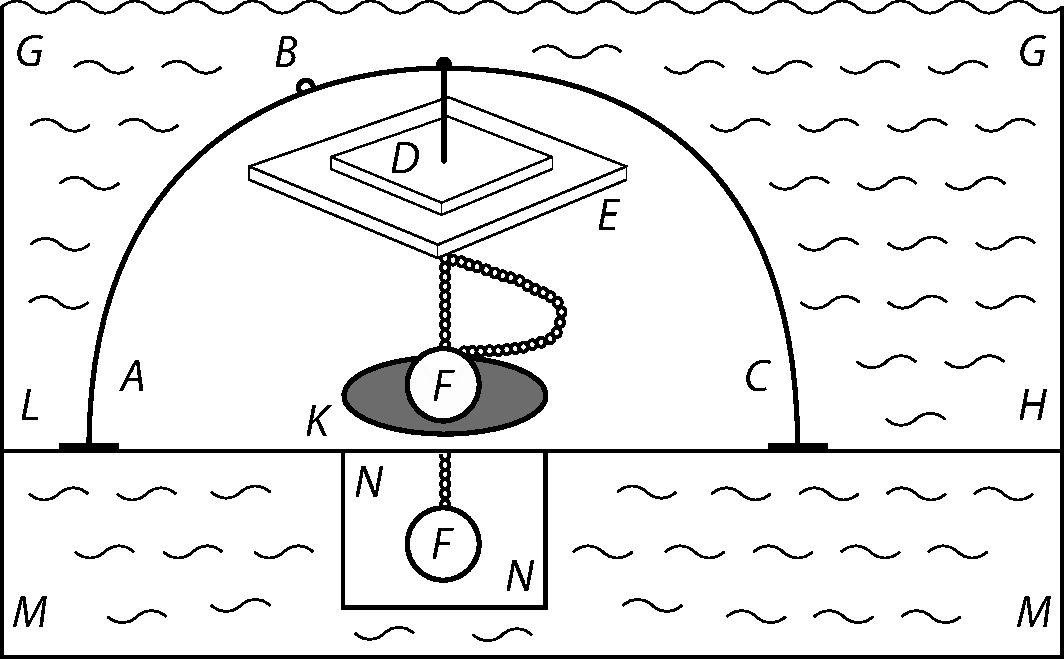
\includegraphics[width=0.69\textwidth]{gesamttex/edit_VIII,3/images/LH_37_03_118r_d.pdf}}%\\
\vspace{0.5em}
\centerline{\lbrack\textit{Fig.~1}\rbrack}%
%
% \newpage%
\count\Bfootins=1200
\count\Afootins=1200
\count\Cfootins=1200
%
% ENDE DES STÜCKES auf Blatt 118r